\documentclass[table, usenames, svgnames, dvipsnames]{beamer}
\usepackage{listings}
\usepackage{beamerthemeshadow}
\usepackage[latin1]{inputenc}
\usepackage[absolute,overlay]{textpos}
\usepackage{array}

% Coisas adicionadas pelo Alberto.
\usepackage{proof}
\usepackage{easylist}
% \usepackage[portuguese]{babel}
\usepackage{amsmath}
\usepackage[round]{natbib}

\usepackage{verbatim}

\usetheme{Rochester}
%\usetheme{Luebeck}
\usecolortheme{rose}

\setbeamerfont{frametitle}{size=\normalsize}
\setbeamerfont{title}{size=\normalsize}
\beamertemplatenavigationsymbolsempty

\setbeamertemplate{navigation symbols}{}
\setbeamertemplate{footline}{}

\DeclareGraphicsExtensions{.pdf,.jpg,.png} % compilamos apenas com pdflatex
\graphicspath{{.}{./figuras/}} % caminho onde as figuras estarao disponiveis

\setlength{\TPHorizModule}{1mm}

\setlength{\TPVertModule}{1mm}
\newcommand{\MyLogo}{%
\begin{textblock}{}(118.5, 2.5)
   
\includegraphics[width=0.7cm]{figuras/ime-mod2.png}
\end{textblock}
}

\title{\footnotesize Subtipos e Metateoria dos Subtipos}

% \usepackage{framed} % utilizado para codigo fonte
\definecolor{shadecolor}{named}{LightGray}

\usepackage[portuguese]{babel}

% ---------------------------------------------------------------------------- %
% T�tulo
% ---------------------------------------------------------------------------- %

\subtitle{}
\date{}

% ---------------------------------------------------------------------------- %
\begin{document}
% ---------------------------------------------------------------------------- %

% ---------------------------------------------------------------------------- %
% Primeira p�gina: slide 0
% --------------------------------------------------------------------------- - %
\begin{frame}
   \centering
   \textsc{Universidade Federal de Santa Maria}\\
   \textsc{Programa de P�s-Gradua��o em Inform�tica - PPGI}\\
   \vspace{15pt}
   \titlepage
   \vspace{-60pt}
   \begin{center}
      \textsc{Linguagens de Programa��o -- ELC921}\\
      \textsc{Prof� Dr� Juliana Kaiser Vizzotto}\\
      \hfill\\
      \textsc{Alunos:} Alberto Kummer, Daniel Di Domenico, Fernando Campagnolo, J�ssica Lasch de Moura e Jos� Puiati
   \end{center}
\end{frame}

%Se��o 15.1
\begin{frame}
   \frametitle{15 Subtyping}
   \begin{itemize}
      \item Tamb�m chamado de \emph{subtype polymorphism};
      \item Caracter�stica presente nas linguagens orientadas a objetos;
      \item C�lculo Lambda simplesmente tipado com subtipos: \Large $\lambda_{<:}$
   \end{itemize}
\end{frame}

\begin{frame}
   \frametitle{15.1 Subsumption}
   \begin{itemize}
      \item Sem subtipos:
         \begin{itemize}
            \item [$\checkmark$] Regras de tipos bastante r�gidas;
            \item [$\checkmark$] Rejei��o de express�es que, aos olhos do programador, s�o bem tipadas.
         \end{itemize}
      \item Exemplo:
   \end{itemize}
   \begin{center}
      $\infer{\Gamma  \vdash t_1 t_2 : T_{11}} {\Gamma  \vdash t_1 : T_{11} \rightarrow T_{12} \qquad \Gamma \vdash t_2 : T_{11}}$ $\qquad \textsc{(T-App)}$ \\
      
      \vspace{0.4in}
      
      $(\lambda{}r\colon\{x:Nat\}. \quad r.x) \quad \{x=0,y=1\}$ \qquad \alt<2>{\textcolor{green}{V�lido}}{Inv�lido?}
   \end{center}   
\end{frame}

\begin{frame}
   \frametitle{15.1 Subsumption}
   \begin{itemize}
      \item Objetivo dos subtipos:
      \begin{itemize}
         \item [$\checkmark$] Refinamento das regras de tipos;
         \item [$\checkmark$] Se S � subtipo de T ($S <: T$), qualquer termo do tipo S pode ser 
                              utilizado no contexto onde T � esperado;
         \item [$\checkmark$] Princ�pio da substitui��o segura (\emph{safe substituition}).                              
      \end{itemize}
   \end{itemize}
   
   \vspace{0.2in}
   
   \begin{block}{Regra \emph{Subsumption}}
      \begin{center}
         $\infer{\Gamma \vdash t : T} {\Gamma \vdash t : S \qquad S <: T}$ $\qquad \textsc{(T-Sub)}$ \\
      \end{center}
   \end{block}
   \small Adaptado de \citep{pierce}.
\end{frame}

\begin{frame}
   \frametitle{15.1 Subsumption}
   \begin{itemize}
      \item Exemplo: $(\lambda{}r\colon\{x:Nat\}. \quad r.x) \quad \{x=0,y=1\}$
      \begin{itemize}
         \setlength\itemsep{0.1in}
         \item [$\checkmark$] Considerando que: $\{x:Nat,y:Nat\} <: \{x:Nat\}$
         \item [$\checkmark$] A regra \textsc{T-Sub} permite a aplica��o pois s�o tipos v�lidos.
      \end{itemize}   
   \end{itemize}   
\end{frame}

%Se��o 15.2
%inicio jessica
\begin{frame}
\frametitle{Tipos de Fun��es}
\begin{itemize}
\item Para construir um tipo que combine booleanos com primitivas do c�lculo lambda � preciso
adicionar uma classifica��o para os termos cuja avalia��o resulta em uma fun��o;
\item A fim de ter certeza de que a fun��o ir� se comportar corretamente quando for chamada, precisamos manter o controle de qual o tipo de argumento que ela espera.
\end{itemize}
\end{frame}

\begin{frame}
\frametitle{Tipos de Funcoes}
\begin{itemize}
\item Para manter esta informa��o, podemos utilizar um novo tipo:
\end{itemize}
\begin{eqnarray*}
    & T ::= \\
    && Bool \\
    && T \to T\\
\end{eqnarray*}
\end{frame}

\begin{frame}
\frametitle{Tipos de Fun��es}
\begin{itemize}
\item Exemplo:
\end{itemize}
\begin{eqnarray*}
    & Bool \to Bool \\
    & (Bool \to Bool) \to (Bool \to Bool) \\
\end{eqnarray*}
\end{frame}

\begin{frame}
\frametitle{Rela��o  de Tipos}
\begin{itemize}
\item Para saber o tipo de uma abstra��o como \textcolor{red}{$"\lambda x.t"$}, precisamos calcular o que acontece quando essa abstra��o � aplicada a algum argumento;
\item Abordagem utilizada agora: anotar a abstra��o com o tipo esperado para seus argumentos.
\item Exemplo: \textcolor{red}{$"\lambda x.t"$} ser� \textcolor{red}{$"\lambda x:T1 .t2"$}
\end{itemize}
\end{frame}

\begin{frame}
\frametitle{Rela��o  de Tipos}
\begin{itemize}
\item Termos podem conter abstra��es aninhadas. Com isso em mente, utilizaremos $\Gamma \vdash t : T$ onde $\Gamma$ � um conjunto com as vari�veis livres de t e seus respectivos tipos. Sendo assim, a regra de tipo para abstra��es ser�:
\end{itemize}
 \begin{center}
{\huge $\frac{\Gamma ,x\ :\ T_1 \vdash t_2\  :\  T_2}{\Gamma\  \vdash\  \lambda x\  :\ T_1 .t_2\  :\  T_1 \to T_2}$}  $\qquad (T-Abs)$
 \end{center}
\end{frame}

\begin{frame}
\frametitle{Rela��o  de Tipos}
\begin{itemize}
\item A regra para vari�vel �:
\end{itemize}
 \begin{center}
{\huge $\frac{x:T\ \in\ \Gamma}{\Gamma\ \vdash\ x\ :\ T}$}  $\qquad (T-Var)$
 \end{center}
 \begin{itemize}
\item A regra para aplica��o �:
\end{itemize}
 \begin{center}
{\huge $\frac{\Gamma\  \vdash\ t_1\ :\ T_{11} \to T_{12} \quad \Gamma\ \vdash\ t_2 : T_{11}}{\Gamma\  \vdash\ t_1\ t_2\ :\ T_{12}}$}  $\qquad (T-App)$
 \end{center}
\end{frame}
%fim jessica


%Se��o 15.4 e 16.4
\begin{frame}
   \frametitle{15.4 The Top and Bottom Types}
   \begin{block}{Formas de subtipos - Top e Bot}
      \footnotesize\emph{Formas sint�ticas:} \\
      \hspace{1.2in} $T ::= ...$ \\
      \hspace{1.5in} $Top$ \\
      \hspace{1.5in} $Bot$ \\
      
      \vspace{0.15in}
      
      \footnotesize\emph{Regras de subtipos:} \\
      \hspace{1.2in} $S <: Top$ $\qquad \textsc{(S-Top)}$ \\
      \vspace{0.1in}      
      \hspace{1.2in} $Bot <: T$ $\qquad \textsc{(S-Bot)}$ \\
      
      \vspace{0.05in}
   \end{block}
   \small Adaptado de \citep{pierce}.
\end{frame}

\begin{frame}
   \frametitle{15.4 The Top and Bottom Types}
   \begin{itemize}
      \setlength\itemsep{0.1in}
      \item Top:
         \begin{itemize}
            \item [$\checkmark$] Elemento \textbf{m�ximo} da rela��o de subtipos;
            \item [$\checkmark$] Equivale ao tipo \emph{Object} das linguagens orientadas a objetos;
            \item [$\checkmark$] Dispositivo t�cnico sofisticado em sistemas que combinam subtipos com poliformismo.
         \end{itemize}

      \item Bot:
         \begin{itemize}
            \item [$\checkmark$] Elemento \textbf{m�nimo} da rela��o de subtipos;
            \item [$\checkmark$] Tipo vazio (n�o existem valores do tipo Bot);
	    \item [$\checkmark$] Muito �til para expressar algumas opera��es que n�o visam retorno de valores, como exce��es, pois:
	    \begin{itemize}
	       \item [--] Permite ao programador definir express�es sem retorno com o tipo Bot;
	       \item [--] Indica ao \emph{typechecker} que a express�o pode ser utilizada com seguran�a em qualquer contexto.
	    \end{itemize}
         \end{itemize}   
   \end{itemize}
\end{frame}

\begin{frame}
   \frametitle{15.4 The Top and Bottom Types}
   \begin{itemize}
      \item Exemplo:
   \end{itemize}
   $\lambda{}x:T.$ \\
   \quad if $<$ valor apropriado para x $>$ then \\
   \quad \quad $<$ calcula o resultado $>$ \\
   \quad else \\
   \quad \quad error
\end{frame}

\begin{frame}
   \frametitle{15.4 The Top and Bottom Types}
   \begin{itemize}
      \item Tipo \texttt{Bot} dificulta a implementa��o;
      \item Mudan�a da regra de tipo da aplica��o:
      \begin{itemize}
         \item [$\checkmark$] \texttt{t1 t2} : 
         \item [$\checkmark$] \texttt{t1} pode ser tanto do tipo seta ($T1 \rightarrow T2$) ou do tipo \texttt{Bot}.
      \end{itemize}
   \end{itemize}
\end{frame}

%Se��o 15.5
\begin{frame}
\frametitle{SLIDES FERNANDO}%A correspond�ncia Curry-Howard}
%\begin{itemize}
%\item Liga��o entre a teoria dos tipos e a l�gica.
%\item S�rie de resultados na fronteira entre a l�gica matem�tica e a teoria da computabilidade de forma a estabelecer uma rela��o entre a demonstra��o formal de um sistema l�gico e um modelo computacional.
%\end{itemize}
\end{frame}

\begin{comment}
\begin{frame}
\frametitle{A correspond�ncia Curry-Howard}
O s�mbolo l�gico "$\to$" vem com regras de dois g�neros:
\begin{enumerate}
\item Uma regra de introdu��o (T-Abs) que descreve como elementos do tipo podem ser criados.
\item Uma regra de elimina��o (T-App), que descreve como os elementos do tipo podem ser usados.
\end{enumerate}
\begin{center}
{\huge $\frac{\Gamma , x : T_1\ \vdash\ t_2 :T_2}{\Gamma\ \vdash\ \lambda x : T_1 . t_2\ :\ T_1\ \to T_2}$} \newline  \newline  \newline
{\huge $\frac{\Gamma\ \vdash\ t_1\ :\ T_{11} \to T_{12} \quad  \Gamma\ \vdash\ t_2\ :\ T_{11}}{\Gamma\ \vdash\ t_1\ t_2\ : T_{12}}$}
\end{center}
\end{frame}

\begin{frame}
\frametitle{A correspond�ncia Curry-Howard}
\begin{itemize}
\item Em L�gicas construtivas a prova de uma proposi��o  P consiste em evidencias concretas para P.
\item Curry e Howard notaram que tais evidencias possuem uma rela��o forte com a  computa��o.
\item Ex.: A prova de uma proposi��o P $\supset$ Q pode ser vista como um procedimento mec�nico que, dada uma prova de P, pode-se construir uma prova de Q. Da mesma forma uma prova P $\land$ Q consiste em uma prova de P em conjunto com uma prova de Q.
\end{itemize}
\end{frame}


\begin{frame}
\frametitle{A correspond�ncia Curry-Howard}
Esta observa��o d� origem a seguinte correspond�ncia:
\begin{figure}[!htb]
\centering
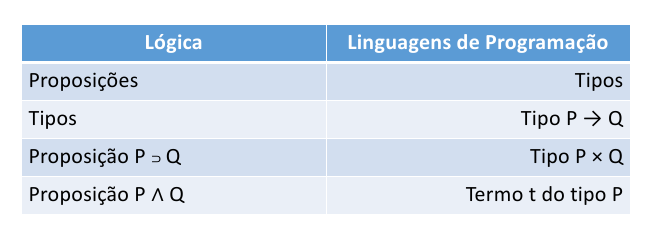
\includegraphics[width=0.65\textwidth]{figuras/tabela.png}
\caption{Tabela}
\label{}
\end{figure}
\end{frame}

\begin{frame}
\frametitle{A correspond�ncia Curry-Howard}
\begin{itemize}
\item A correspond�ncia Curry-Howard n�o �  limitada para um sistema de um tipo particular e uma logica espec�fica, pelo contrario pode ser estendido a uma enorme variedade de sistemas de tipos e l�gicas.
\end{itemize}
\end{frame}

\begin{frame}
\frametitle{Corre��o e Tipagem}
\begin{itemize}
\item Anota��es de tipo n�o desempenham qualquer papel na avalia��o.
\item A maioria dos compiladores para linguagens de programa��o em grande escala, evitam mostrar coment�rios em tempo de execu��o: eles s�o usados durante o typechecking (e durante a gera��o de c�digo, em compiladores mais sofisticados).
\item Tipos n�o aparecem no c�lculo lambda simplesmente tipado na sua forma compilada. Os programas s�o convertidos para uma forma sem tipos antes de serem avaliadas.

\end{itemize}
\end{frame}


\end{comment}


%Se��o 15.6 e 15.7
\begin{frame}
   \frametitle{15.6 Sem�ntica de coer��o para sistema de subtipos}
   \begin{itemize}
      \item Subtipos fornecem ao programador uma maior flexibilidade na escrita do c�digo, \textbf{o que pode ocasionar alguma sobrecarga em tempo de execu��o}
      \begin{itemize}
         \item [$\times$] seja por consequ�ncia da representa��o de dados em uma m�quina real
         \begin{align*}
            \texttt{Int} \subtype \texttt{Float} & &
         \end{align*}
         \item [$\times$] ou pela natureza das linguagens de programa��o funcionais
         \begin{align*}
            \texttt{\{l}_i \texttt{=} \texttt{v}_i ~^ {i \in 1..n}\texttt{\}}.\texttt{l}_j \rightarrow \texttt{v}_i
               & & \mbox{\rulename{(E-ProjRcd)}}
         \end{align*}
      \end{itemize}
   \end{itemize}
\end{frame}

\begin{frame}
   \frametitle{15.6 Sem�ntica de coer��o para sistema de subtipos}
   \textbf{Sem�nticas de coer��o}\\
   \begin{itemize}
      \item Ideia principal: \textbf{substituir} express�es que envolvem subtipos por express�es de mais ``baixo n�vel''
      \begin{itemize}
         \item [$\checkmark$] processo que ocorre em tempo de execu��o
         \item [$\checkmark$] geralmente as express�es s�o compiladas para uma linguagem pr�xima a de m�quina
      \end{itemize}
      \item Tudo em raz�o da performance:
      \begin{itemize}
         \item [$\checkmark$]  reduzir a necessidade de \textbf{buscas} durante a execu��o de c�digo
      \end{itemize}
      \item No livro-texto da disciplina
      \begin{itemize}
         \item [$\checkmark$]  Linguagem utilizada pelo programador: $\lambda_{\hspace{-4pt}\textttf{\subtype}}$ %C�lculo lambda simplesmente tipado com subtipos e registros
         \item [$\checkmark$]  Linguagem de baixo n�vel: $\lambda_{\rightarrow}$ %C�lculo lambda puro com registros e tipo \texttt{Unit}
      \end{itemize}
   \end{itemize}
\end{frame}

\begin{frame}
   \frametitle{15.6 Sem�ntica de coer��o para sistema de subtipos}
   \textbf{Sem�nticas de coer��o}\\
   \begin{itemize}
      \item � vista como uma fun��o que \textbf{toma um tipo e devolve outro}
      \item � expressa por \obrack---\cbrack
      \begin{align*}
         & \mbox{\textttf{\obrack Top\cbrack}} & &= \mbox{\textttf{Unit}}\\
         & \mbox{\textttf{\obrack T$_1\rightarrow$ T$_2$\cbrack}} & &= \mbox{\obrack \textttf{T$_1$}\cbrack $\rightarrow$ \obrack \textttf{T$_2$}\cbrack}\\
         & \mbox{\textttf{\obrack \{l$_i$:T$_i~^{i \in 1..n}$\}\cbrack}} &
            & = \mbox{\{\textttf{l$_i$:\obrack T$_i$\cbrack $^{i \in 1..n}$}\}}
      \end{align*}
   \end{itemize}
\end{frame}

\begin{frame}
   \frametitle{15.6 Sem�ntica de coer��o para sistema de subtipos}
   \textbf{Sem�nticas de coer��o}\\
   \begin{itemize}
      \item Em tempo de execu��o as coer��es s�o inseridas nos locais onde ocorrem \textit{subsumptions}
      \item \cite{pierce} sugere a formaliza��o de coer��es como \textbf{fun��es de deriva��o de tipos}
   \end{itemize}
   \begin{align*}
      \mathcal{C} \ \mathrm{::} \ & \mbox{\textttf{S \subtype T}}\\
      \mathcal{D} \ \mathrm{::} \ & \mbox{\textttf{$\Gamma \vdash $ t:T}}
   \end{align*}
\end{frame}

\begin{frame}
   \frametitle{15.6 Sem�ntica de coer��o para sistema de subtipos}
   \textbf{Sem�nticas de coer��o}\\
   \begin{itemize}
      \item Mas n�o basta saber que \textttf{S\subtype T}
      \begin{itemize}
         \item [$\checkmark$] n�o basta inventar uma regra e adot�-la
         \item [$\checkmark$] as regras de subtipagem justificam o emprego das coer��es
         \item [$\checkmark$] interpretadas como \textbf{�rvores de deriva��o de subtipos}
      \end{itemize}
   \end{itemize}
   \begin{align*}
      & \textttf{\huge\obrack} \mbox{
         \infer [\rulename{\scriptsize(S-Refl)}] {\textttf{T\subtype T}} {}
      } \textttf{\huge\cbrack} & & =  \lambda \textttf{x:\obrack T\cbrack .x}
      \\
      & \textttf{\Huge\obrack} \mbox{\scriptsize
         \infer [\rulename{\scriptsize(S-Trans)}] {\textttf{S\subtype T}} {
            \textttf{$\mathcal{C}_1\ \mathrm{::}\ $S\subtype U} & \quad \textttf{$\mathcal{C}_2\ \mathrm{::}\ $U\subtype T} &
         }
      } \textttf{\Huge\cbrack} & & =  \lambda \textttf{x:\obrack S\cbrack .\obrack $\mathcal{C}_2$\cbrack(\obrack $\mathcal{C}_1$\cbrack\ x)}
   \end{align*}
 \end{frame}

\begin{frame}
   \frametitle{15.6 Sem�ntica de coer��o para sistema de subtipos}
   \textbf{Sem�nticas de coer��o}\\
   \begin{itemize}
      \item \textbf{Lema:} Se $\mathcal{C}\ \mathrm{::}\ $ \textttf{S\subtype T}, ent�o
         $\vdash$ \textttf{\obrack}$\mathcal{C}$\textttf{\cbrack\ :}
         \textttf{\obrack S\cbrack\ $\rightarrow$ \obrack T\cbrack}
      \begin{flushright}
         $\square$
      \end{flushright}
   \end{itemize}
\end{frame}

\begin{frame}
   \frametitle{15.6 Sem�ntica de coer��o para sistema de subtipos}
   \textbf{Sem�nticas de coer��o}\\
   \begin{itemize}
      \item Coer��es interagem com o contexto de tipos
      \begin{itemize}
         \item [$\checkmark$] interpretadas como \textbf{deriva��es de tipos}
      \end{itemize}
   \end{itemize}
   \begin{align*}
      & \textttf{\Huge\obrack} \mbox{\scriptsize
         \infer [\rulename{\scriptsize(T-Sub)}] {\textttf{$\Gamma \vdash$ t : T}} {
            \textttf{$\mathcal{D}\ \mathrm{::}\ \Gamma \vdash\ $t : S} & \quad \textttf{$\mathcal{C}\ \mathrm{::}\ $S\subtype T} &
         }
      } \textttf{\Huge\cbrack} & & = & \textttf{\obrack $\mathcal{C}$\cbrack \obrack $\mathcal{D}$\cbrack}
   \end{align*}
\end{frame}

\begin{frame}
   \frametitle{15.6 Sem�ntica de coer��o para sistema de subtipos}
   \textbf{Sem�nticas de coer��o}\\
   \begin{itemize}
      \item \textbf{Teorema:} Se $\mathcal{D}\ \mathrm{::}\ \vdash $ \textttf{t : T}, ent�o
         \textttf{\obrack $\Gamma$\cbrack} � a extens�o ponto a ponto entre os contextos de tipos
         \textttf{\obrack $\varnothing$\cbrack\ = $\varnothing$} e \\ \texttt{\obrack $\Gamma$, x:T\cbrack\ = \obrack $\Gamma$\cbrack, x:\obrack T\cbrack}
      \begin{flushright}
         $\square$
      \end{flushright}
   \end{itemize}
\end{frame}

\begin{frame}
   \frametitle{15.6 Sem�ntica de coer��o para sistema de subtipos}
   \textbf{Sem�nticas de coer��o}\\
   \begin{itemize}
      \item Cuidado com a \textbf{coer�ncia}
      \begin{itemize}
         \item [$\checkmark$] Deriva��o de tipos n�o deve incluir ambiguidades na linguagem
      \end{itemize}
      \item \textbf{Defini��o: } Uma tradu��o \obrack ---\cbrack\ para a deriva��o de tipos de uma linguagem para termos de outra � coerente se, para cada par de deriva��es $\mathcal{D}_1$ e $\mathcal{D}_2$ com a mesma conclus�o $\Gamma \vdash$ \textttf{t:T}, as tradu��es \texttt{\obrack} $\mathcal{D}_1$\texttt{\cbrack} e \texttt{\obrack} $\mathcal{D}_2$\texttt{\cbrack} apresentam o mesmo comportamento na liguagem de destino.
   \end{itemize}
\end{frame}









\begin{frame}
   \frametitle{15.7 Os tipos Interse��o e Uni�o}
   \begin{align*}
   & \mbox{
      \textttf{T$_1$ $\wedge$ T$_2$ \subtype\ T$_1$}
   } & & \mbox{\rulename{(S-Inter1)}}\\
   & \mbox{
      \textttf{T$_1$ $\wedge$ T$_2$ \subtype\ T$_2$}
   } & & \mbox{\rulename{(S-Inter2)}}\\
   & \mbox{
      \infer {\textttf{S \subtype\ T$_1$ $\wedge$ T$_2$}} {
         \textttf{S \subtype\ T$_1$} & \textttf{S \subtype\ T$_2$}
      }
   } & & \mbox{\rulename{(S-Inter3)}}\\
   & \mbox{
      \textttf{S $\rightarrow$ T$_1$ $\wedge$ S $\rightarrow$ T$_2$ \subtype\ S $\rightarrow$ (T$_1$ $\wedge$ T$_2$)}
   } & & \mbox{\rulename{(S-Inter4)}}
   \end{align*}
   \begin{itemize}
      \item [] De forma semelhante para o tipo \textbf{Uni�o}
   \end{itemize}
\end{frame}



% \begin{block}{}
%    \centering
%    \texttt{\frenchspacing($\lambda$x:\{y: Nat\}.x.y) \{x: 4, y: 8\}}
% \end{block}
% \infer [\rulename{S-Trans}] {\textttf{\{x: Nat, y: Nat\} \subtype  \{y: Nat\}}} {
%    \infer [\rulename{S-RcdPerm}] {
%       \begin{array}{@{}c}
%          \textttf{\{y: Nat, x: Nat\}} \\ \subtype \textttf{\{x: Nat, y: Nat\}}
%       \end{array}
%    } {} &
%    \infer [\textsc{S-RcdWidth}] {
%       \begin{array}{@{}c}
%          \textttf{\{y: Nat, x: Nat\}} \\ \subtype \textttf{\{y: Nat\}}
%       \end{array}
%    } {}
% }


%Se��o 16, 16.1 e 16.2
%in�cio kadico
\begin{frame}{SLIDES KADICO}% 9.3.1 - Lemma [Inversion of the typing relation]}
  %\begin{itemize}
  %\item {
  %  If $\Gamma \vdash x : R$ , then $x : R \in \Gamma$.
  %}
  %\item {
  %  If $\Gamma \vdash \lambda x : T_1 . t_2 : R$ , then $R : T_1 \rightarrow R_2$ for some $R_2$ with $\Gamma, x : T1 \vdash t_2 : R_2$.
  %}
  %\item {
  %  If $\Gamma \vdash$ $t_1$ $t_2 : R$ , then there is some type $T_{11}$ for some $R_2$ with $\Gamma, x : T_1 \vdash t_2 : R_2$.
  %}
  %\item {
  %  If $\Gamma \vdash true : Bool$ , then $R : Bool$.
  %}
  %\item {
  %  If $\Gamma \vdash false : Bool$ , then $R : Bool$.
  %}
  %\item {
  %  If $\Gamma \vdash $ if then $ t_2  $ else $ t_3 : R$ , then $\Gamma \vdash t_1 : Bool$ and $t_1$  $t_2 : R$.
  %}
  %\end{itemize}
\end{frame}

\begin{comment}
\begin{frame}{9.3.3 - Theorem [Uniqueness of Types]}
  \begin{itemize}
  \item {
    Give a context $\Gamma$ and a Term t, t must have at most one type.
  }
  \item {
    [Proof] If $\Gamma \vdash x : T$ and $\Gamma \vdash x : S$ then S = T by T-Var.
  }
  \end{itemize}
\end{frame}

\begin{frame}{9.3.4 - Lemma [Canonical Forms]}
  \begin{itemize}
  \item {
    If v : Bool, then v is $true \mid false$.
  }
  \item {
    If v : $T_1 \rightarrow T_2$ , then $v = \lambda x : T_1 . t_2$.
  }
  \end{itemize}
\end{frame}

\begin{frame}{9.3.5 - Theorem [Progress]}

  \begin{itemize}
  \item {
     If $\vdash k : T$ then either k is a value, or $k \rightarrow k'$ to some k'.
  }
  \item {
     The variable case cannot occur.
  }
  \item {
     The abstraction occur, since abstractions are values.
  }
  \item {
     The application is not so simple.
     \begin{itemize}
      \item {
         Case T-App: $k' = k_1$  $k_2$  $\mid$  $\vdash k_1 : T_{11} \rightarrow T_{12}$ and $k_2 : T_{11}$.
      }
      \item {
         $k_1$ is a term or it can make a step, in the same way $k_2$.
      }
      \item {
         If $k_1$ can make a step, then applies E-App1.
      }
      \item {
         If $k_1$ is a value and $k_2$ can make a step, then applies E-App2.
      }
      \item {
         If booth are value, then the canonical form of $k_1$ is $\lambda x : T_{11} . k_{12}$, and applies E-AppAbs.
      }
     \end{itemize}
  }
  \end{itemize}
\end{frame}

\begin{frame}{9.3.6 - Lemma [Permutation]}
  \begin{itemize}
  \item {
   If $\Gamma \vdash e : T$ and $\Gamma'$ is a permutation of $\Gamma$, then $\Gamma' \vdash e : T$.
  }
  \item {
   Proof: $\Gamma \vdash e : T$
  }
  \end{itemize}
\end{frame}

\begin{frame}{9.3.7 - Lemma [Weakening]}
  \begin{itemize}
  \item {
     If $\Gamma \vdash e : T$ and $x \not\in dom(\Gamma)$, then $\Gamma, x : S \vdash t : T$.
  }
  \item {
   Proof: $\Gamma \vdash e : T$
  }
  \end{itemize}
\end{frame}

\begin{frame}{9.3.8 - Lemma [Preservation of Types Under the Substitution][1]}
  \begin{itemize}
  \item {
    If $\Gamma, x : T' \vdash e : T$, and $\Gamma \vdash e' : T'$, then $\Gamma \vdash [x \rightarrow e'] e : T$
  }
  \item {
   Proof: If $\Gamma, x : T' \vdash e : T$.
 }
  \item[?] {Case T-Var:}

   \begin{itemize}
   \item[?] \textbf{t = z with z : T $\in$ ($\Gamma$, x : S)}
   \item {
      If $z = x$, then $[x \rightarrow s] z = s$
    }
    \item {
      Otherwise, $[x \rightarrow s] z = z$
     }
     \end{itemize}

  \item[?] {Case T-Abs}
   \begin{itemize}
   \item[?] \textbf{t = $\lambda$ y : $T_2$ . $t_1$ \\
               T = $T_2 \rightarrow T_1$ \\
               $\Gamma$ x : S, y : $T_2 \vdash t_2 : T_1$
               }
   \item {
      $x \not= y$, and $y \not\in FV(s)$.
    }
    \item {
      Permutation $\Gamma y : T_2, x : S \vdash t_1 : T_1$
     }
     \item {
      Weakening $\Gamma, y : T_2 \vdash s : S$
     }
     \item {
      By induction $\Gamma, y : T_2 \vdash [x \rightarrow s] t_1 : T_1$
     }
     \item {
      By T-Abs $\Gamma \vdash \lambda y : T_2 . [x \rightarrow s] t_1 : T_2 \rightarrow T_1$
     }
     \end{itemize}

  \end{itemize}
  \end{frame}
\begin{frame}{9.3.8 - Lemma [Preservation of Types Under the Substitution][2]}
  \begin{itemize}
  \item[?] {Case T-App:}

   \begin{itemize}
   \footnotesize
      \item {
      By induction $\Gamma \vdash [x \rightarrow s] t_1 : T_2 \rightarrow T_1$ \\
      and $\Gamma \vdash [x \rightarrow s] t_2 : T_2$
     }
     \item {
      By T-App $\Gamma \vdash [x \rightarrow s] t_1 [x \rightarrow s] t_2 : T$
     }
   \end{itemize}

  \item[?] {Case T-True and T-False}
   \begin{itemize}
   \item[?] \textbf{t = true \\
                t = false \\
                T = Bool}
   \item {
      $ [x \rightarrow s] t = (true \mid false)$, $\Gamma \vdash [x \rightarrow s] t : T$
    }
     \end{itemize}
     \item[?] {Case T-If}
      \begin{itemize}
      \item[?] \textbf{t = if $t_1$ the $t_2$ else $t_3$\\
                $\Gamma$ x : S $\vdash t_1$ : Bool \\
                $\Gamma$ x : S $\vdash t_2$ : T \\
                $\Gamma$ x : S $\vdash t_3$ : T}
      \item {
        By induction we have: \\
        $\Gamma \vdash [x \rightarrow s] t_1$ : Bool \\
        $\Gamma \vdash [x \rightarrow s] t_2$ : T \\
        $\Gamma \vdash [x \rightarrow s] t_2$ : T \\
      }
     \end{itemize}

  \end{itemize}
  \normalsize
\end{frame}

\begin{frame}{9.3.9 - Theorem [Preservation]}
  \begin{itemize}
  \item {
    If $\Gamma \vdash e : T$ and $e \rightarrow e'$, then $\Gamma e' : T$.
  }
  \end{itemize}
\end{frame}

\end{comment}

\bibliography{referencias}
\bibliographystyle{plainnat}

\end{document}
